\section{Tecnologías implementadas y estado operativo.}
\subsection{Análisis de RAM}
\label{subsec:ramanalisi}
Uno de los puntos más importantes a la hora de implementar un bot con IA para un juego de Atari, es entender cómo está hecho. Utilizaremos el entorno \ac{ale} para extraer características de los juegos, el cual cuenta con una API que nos permite extraer información de los mismos. Para ello, se ha desarrollado un lector de RAM que nos ayuda a visualizar los 128 bytes de memoria de la Atari mientras se ejecuta un juego.

Además, dicho lector implementa colores, lo cual permite que se puedan distinguir las posiciones de RAM que cambian de las que no en un step determinado (paso de ejecución)  como se puede ver en la figura \ref{fig:RAM_Colors}.

\begin{figure}[h]
	\centering
	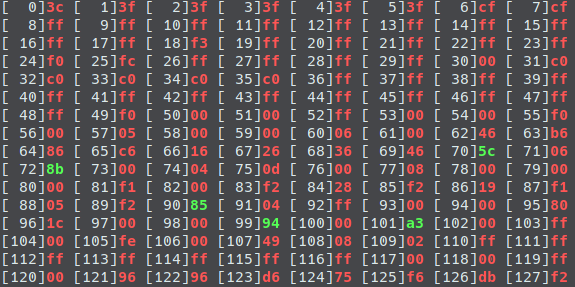
\includegraphics[width=0.95\textwidth]{Figures/RAMColors}
	\caption{El color verde indica que el valor ha cambiado en este step.}
	\label{fig:RAM_Colors}
\end{figure}

Una de las características de este lector es que acompaña la ejecución con un volcado de analytics para ver las posiciones de RAM que más han cambiado en una ejecución determinada.

Para extraer los datos mas interesantes de un juego en concreto, simplemente hay que observar las posiciones de RAM mas alteradas según nuestro analytics. Una vez hecho esto, se pondrá el juego en cámara lenta gracias a una feature del entorno \ac{ale}, lo cual nos permitirá ver con qué sentido cambian estos valores. Como punto a destacar, no todos los valores que cambian mucho serán relevantes a la hora de sacar datos importantes del juego (un contador podría no ser relevante para un caso específico).

Una vez hecho esto se puede desglosar la RAM de manera bastante precisa, sacando datos como los siguientes.

\begin{figure}[h]
	\centering
	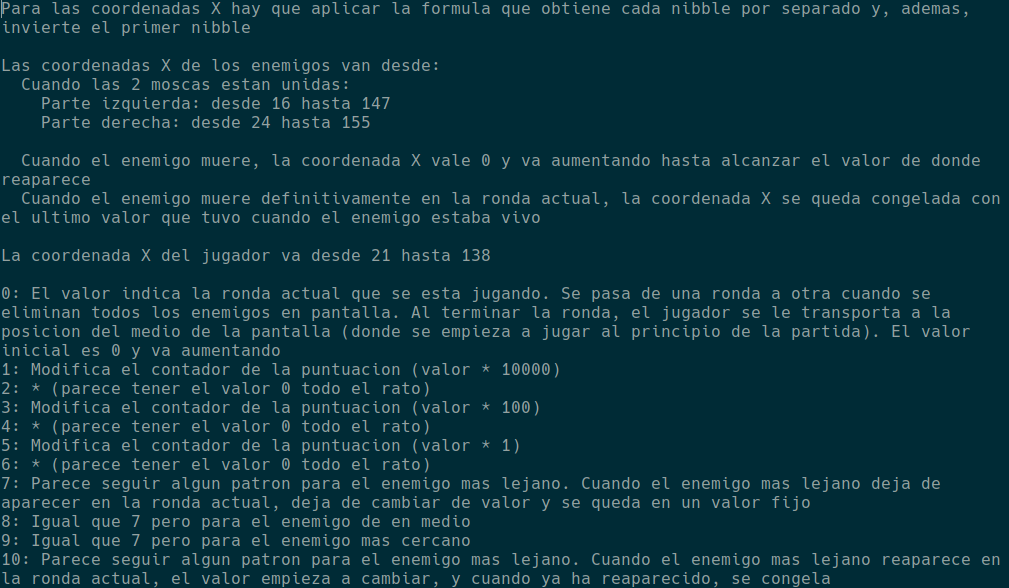
\includegraphics[width=1\textwidth]{Figures/AnalisisRAM}
	\caption{Demon Attack - Análisis de las primeras posiciones de RAM}
	\label{fig:AnalisisRAM}
\end{figure}

Como se puede observar en la figura \ref{fig:AnalisisRAM}, para obtener la información correcta no solo basta con extraer las posiciones relevantes, en algunos casos será necesario procesar esta información. Por ejemplo, en Demon Attack, las coordenadas X de las entidades aparecen ofuscadas de la siguiente manera:

\begin{figure}[h]
	\centering
	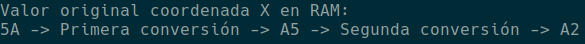
\includegraphics[width=1\textwidth]{Figures/DAttackOpsRequired}
	\caption{Demon Attack - Coordenadas X de las entidades}
	\label{fig:DAttackOpsRequired}
\end{figure}

Como podemos ver en la figura \ref{fig:DAttackOpsRequired}, los nibbles de las coordenadas están invertidos, además, el primer nibble requiere una operación extra, una resta (7 - valor del nibble). 

Una vez tenemos la información recogida y procesada, la podremos utilizar para crear una IA capaz de jugar al juego en concreto. Además de eso, el entorno \ac{ale} cuenta con diversas funcionalidades que nos permiten recoger la información en pantalla en el caso que fuese necesario. 

\subsubsection{Modificando ALE}
\label{subsubsec:ramanalisi:modale}

La primera aproximación que se hizo a la hora de analizar los datos de los diferentes juegos fue básica y útil, pero presentaba varios problemas. El problema más serio que nos encontramos era la cantidad de datos que teníamos ante nuestros ojos, cosa que puede dificultar bastante el encontrar la información importante que necesitamos y, además, que dependemos totalmente de nuestra "intuición" para saber que significa cierta posición de la RAM. Intentando solventar un poco este problema, se nos ocurrió aislar las posiciones que hay en la RAM y, además, poder modificar esos valores aislados para no depender totalmente de nuestra intuición, sino saber más a ciencia cierta, a base de prueba y error, saber qué hace cierta posición de RAM, lo cual nos daría la ventaja de profundizar más en aquellas posiciones de RAM que por alguna razón, en el paso anterior, hemos visto que podían resultar relevantes.

A la hora de intentar poner esta idea en práctica lo primero que intentamos es obtener una referencia de la RAM desde el objeto que hemos ido empleando en todo momento: \textbf{ALEInterface}. Este objeto nos dota del método \textit{getRAM()} que hemos ido utilizando en todo momento para el análisis de los datos (y para posteriormente el tratamiento de los mismos) y que está en el archivo \textit{src/ale\_interface.cpp}. La implementación de dicho método es la siguiente:

\begin{figure}[h]
	\centering
	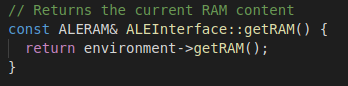
\includegraphics[width=1\textwidth]{Figures/methodGetRAM}
	\caption{Método \textit{getRAM()}}
	\label{fig:methodGetRAM}
\end{figure}

Como observamos, el método \textit{getRAM()} nos devuelve una referencia de un objeto de tipo \textbf{ALERAM}, por lo que vamos a ver que método nos pueden servir para modificar la RAM. Cuando investigamos el archivo \textit{src/environ-ment/ale\_ram.hpp} encontramos la definición del objeto ALERAM y la implementación de sus métodos. Contiene 2 métodos que pueden servirnos para nuestro propósito (modificar la RAM), los cuales se muestran en la figura \ref{fig:ALEMethodsToGetReferencesToRAM}.

\begin{figure}[h]
	\centering
	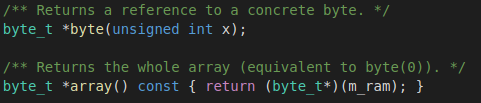
\includegraphics[width=1\textwidth]{Figures/ALEMethodsToGetReferencesToRAM}
	\caption{Métodos de acceso a la RAM de ALEInteface}
	\label{fig:ALEMethodsToGetReferencesToRAM}
\end{figure}

\newpage
Una vez ya encontramos estos métodos, intentamos hacer una pequeña prueba, la cual falla, ya que al intentar hacer uso del método \textit{array()} vemos que modificamos un valor y que, efectivamente, al volver a comprobar el valor, se ha modificado, pero nada sucede en el juego (la prueba la realizamos sobre el videojuego \textit{breakout}, el cual tiene la coordenada X de la barra en la posición 72). Lo que estaba sucediendo, después de indagar un poco por el código de ALE era que el método \textit{getRAM()} de \textit{ale\_interface.cpp} era un método que a su vez llamaba a otro método llamado \textit{getRAM()} pero del objeto \textbf{StellaEnvironment}, objecto que es el encargado de manejar todo el entorno de ALE. Este objeto, de nuevo, devuelve otra vez un objeto de tipo ALERAM por referencia, por lo que de nuevo parece que no hay problema, pero este objeto, \textit{StellaEnvironment}, contiene una copia de la RAM del objeto \textbf{OSystem}, objeto que es el núcleo de la Atari 2600 (del emulador). El problema consiste en que este objeto ALERAM con el que constantemente trabajamos es una copia del que el objeto \textit{OSystem} contiene, es decir, cada vez que llamados al método \textit{getRAM()} desde \textit{ale\_interface.hpp}, se hace otra llamada al método \textit{getRAM()} de \textit{src/environment/stella\_environment.cpp} y este devuelve su copia interna, no la del núcleo de la consola. Cada vez que el objeto \textit{StellaEnvironment} actualiza su copia hace uso del método \textit{processRAM()}.

\begin{figure}[h]
	\centering
	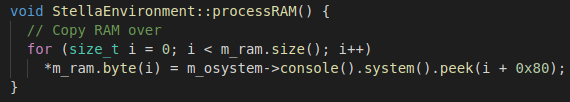
\includegraphics[width=1\textwidth]{Figures/StellaEnviromentProcessRAMMethod}
	\caption{Método \textit{processRAM()} de StellaEnviroment}
	\label{fig:StellaEnviromentProcessRAMMethod}
\end{figure}

Una vez llegado a este punto, lo que se puede hacer si se quiere modificar la RAM que contiene el objeto \textit{OSystem} es implementar un método que lo que haga es actualizar la RAM del objeto \textit{OSystem} del mismo método que que podemos observar que se puede obtener una copia de la RAM con su método \textit{console().system().peek()}, pero tenemos que comprobar si existe el método que nosotros necesitamos, y es que en vez de \textit{peek()} necesitamos un método que nos permita actualizar. De nuevo, buscando en el código, encontramos el archivo \textit{src/emucore/OSystem.hxx}, el cual nos lleva al archivo \textit{src/emucore/Console.hxx}, el cual nos lleva, finalmente, al archivo \textit{src/emucore/System.hxx}. En este último encontramos el método \textit{poke(uInt16, uInt8)}, el cual nos indica a través de su descripción que modifica un valor de la RAM de la consola Atari 2600. Parece ser que ya lo tenemos todo, pero nos queda un último problema, y es que este método no es accesible desde el objeto \textit{StellaEnvironment}, ya que su referencia del objeto \textit{OSystem}, a diferencia del objeto \textit{ALEInterface}, está en su parte privada y no nos da ningún método público para obtener una copia de la referencia. El último paso que nos queda para solucionar este último problema es modificar el código y añadir un método que nos permita actualizar la RAM de la Atari 2600 a partir de la copia que tiene internamente el objeto \textit{StellaEnvironment}, ya que esta última sí que podemos modificarla.

\begin{figure}[h]
	\centering
	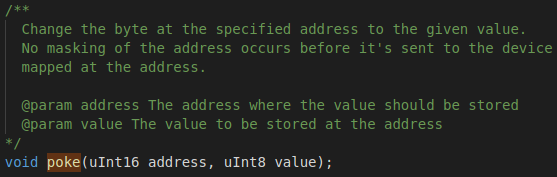
\includegraphics[width=1\textwidth,height=30mm]{Figures/pokeMethod}
	\caption{Método \textit{poke(uInt16, uInt8)}}
	\label{fig:pokeMethod}
\end{figure}

El método que hemos implementado es muy sencillo. Es igual que el método \textit{processRAM()} pero utilizando el método \textit{poke()} en vez de \textit{peek()}. Una vez ya implementado el método, simplemente implementamos otro método en el objeto \textit{ALEInterface} que simplemente haga una llamada a este método que está en el objeto \textit{StellaEnvironment} y ya habremos actualizado la RAM de la Atari 2600. Por último solo quedaría recompilar ALE. Este proceso que hemos realizado a sido con el único objetivo de comprender mejor el significado de las posiciones de RAM de los diferentes juegos a analizar durante este trabajo. Se adjuntarán para cada juego un archivo denominado \textbf{RAM.txt} en el cual hemos analizado cada posición de RAM de manera aislada.

\begin{figure}[h]
	\centering
	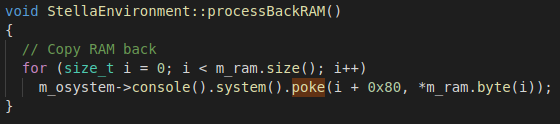
\includegraphics[width=1\textwidth,height=23mm]{Figures/processBackRAM}
	\caption{Método que actualiza la RAM de la Atari 2600}
	\label{fig:processBackRAM}
\end{figure}

\newpage
\subsection{Bots básicos}
\label{subsec:botsbasicos}
Se han desarrollado bots semi-deterministas empleando técnicas básicas de inteligencia artificial para poder extraer datos de gameplay. Los primeros volcados de datos se hicieron con operarios humanos jugando a los juegos, pero al ver que nuestras scores eran mas bien bajas, se optó por implementar IA básica para cada uno de los juegos. 

Estas implementaciones básicas mejoraron mucho las scores obtenidas, por lo que los datos extraídos de los bots eran mas afines a obtener mayores puntuaciones que los nuestros.

Además, sobre esta IA básica, se pueden hacer iteraciones de mejora, teniendo en cuenta más datos o mas información en pantalla, como se ha comentado anteriormente en la subsección \ref{subsec:ramanalisi}.

Este scripting básico ayudará mas adelante a la implementación utilizando machine learning, ya que los datos extraídos y procesados para la implementación básica serán utilizados por el algoritmo de machine learning.

A continuación, describiremos cada uno de los bots básicos y su funcionamiento al igual que algunos detalles de implementación.

\subsubsection{Plantilla común}
\label{subsec:botsbasicos:plantcomun}
Todos los bots comparten una serie de utils que analizaremos a continuación.

\begin{figure}[h]
	\centering
	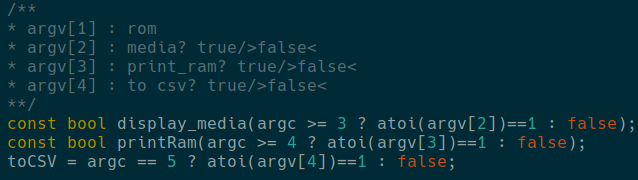
\includegraphics[width=1\textwidth]{Figures/ALEMediaSettings}
	\caption{Opciones de ejecución}
	\label{fig:ALEMediaSettings}
\end{figure}

argv 1 es la ROM que utilizará nuestro ejecutable, argv 2 se corresponde con el contenido multimedia (video y audio), argv 3 escribirá la RAM en consola y argv 4 exportará los datos de gameplay a un archivo \ac{csv} si así se requiere. Se han parametrizado estas opciones porque las ejecuciones son mucho mas lentas conforme mas información requiramos, esto se nota sobre todo a la hora de desactivar el contenido multimedia.

\begin{figure}[h]
	\centering
	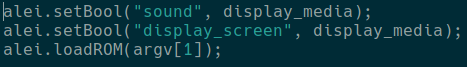
\includegraphics[width=0.7\textwidth]{Figures/ALEromANDmedia}
	\caption{La ROM y el contenido multimedia corren a cargo de \ac{ale}.}
	\label{fig:ALEromANDmedia}
\end{figure}

\newpage
Algunas de estas opciones corren a cargo del entorno (Figura 	\ref{fig:ALEromANDmedia}), mientras que las otras han sido implementadas por nosotros.

Otra de las partes comunes a todos los bots es el bucle principal de ejecución que podemos ver a continuación en la figura \ref{fig:ALEMainExecLoop}. Este bucle está situado en \textbf{main()} y es el encargado de analizar y ejecutar las acciones requeridas en cada step del juego en activo.

\begin{figure}[h]
	\centering
	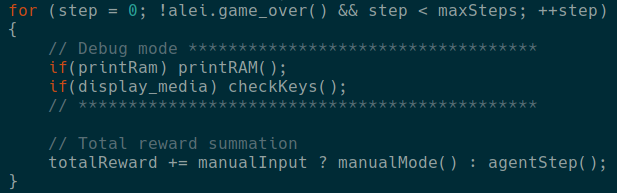
\includegraphics[width=0.95\textwidth]{Figures/ALEMainExecLoop}
	\caption{Bucle principal de ejecución.}
	\label{fig:ALEMainExecLoop}
\end{figure}

En este bucle observamos nuestra opción \textbf{printRam} que llama al método encargado de imprimir la RAM, el cual convierte a hexadecimal cada uno de los valores de RAM obtenidos mediante el método \textbf{getRAM().get(i)} del entorno \ac{ale}, además hace un seguimiento de los valores de RAM del step anterior para comprobar si dichos valores han cambiado como hemos visto anteriormente en la figura \ref{fig:RAM_Colors}.

Otra opción que encontramos en el bucle principal de ejecución es \textbf{display\_media}, pero en este caso es usado para llamar al método \textbf{checkKeys()}, esto se hace porque no tiene sentido trackear el input si no existe contenido de video. Este método de input es propio, ya que el método de input de ALE "pausa" el agente, lo cual no nos interesa para extraer datos. \textbf{checkKeys()} simplemente activa o desactiva el modo manual propio con la tecla "E", reflejado en la variable \textbf{manualInput}.

La variable \textbf{manualInput} decidirá que función se llama para calcular \textbf{totalReward}. \textbf{manualMode()} mapea el teclado a diferentes acciones del juego, mientras que \textbf{agentStep()} es el bot autónomo específico a cada juego.

Otra de las partes comunes a todos los agentes es la parte de volcado de datos, para ello se han implementado dos funciones de escritura que imprimen strings o dobles en el archivo \ac{csv} anteriormente comentado, como bien podemos ver en la figura .

\begin{figure}[h]
	\centering
	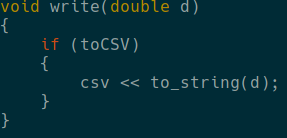
\includegraphics[width=0.4\textwidth]{Figures/aledumpcsv}
	\caption{Una de las funciones de escritura en CSV.}
	\label{fig:aledumpcsv}
\end{figure}


\subsubsection{Breakout}
\label{subsec:botsbasicos:breakout}
El Breakout es el juego mas simple de todos los que analizaremos en esta parte de la sección, pues el número de inputs que tiene es mas bien pequeño. En el Breakout contamos con un total de 5 vidas para pasarnos los 2 niveles de los que dispone. El Breakout fue el primer juego en el que vimos la necesidad de automatizar al jugador, ya que la velocidad de la pelota va incrementando en función a los ladrillos restantes que quedan, lo cual provocaba que perdiésemos siempre en este punto.

\begin{figure}[h]
	\centering
	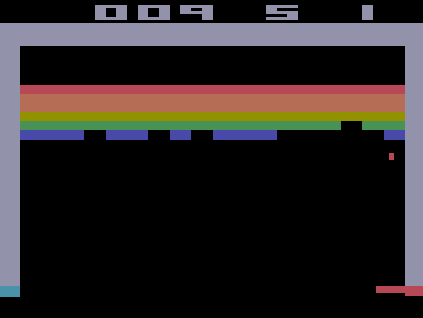
\includegraphics[width=0.7\textwidth]{Figures/breakoutgame}
	\caption{Juego Breakout.}
	\label{fig:breakoutgame}
\end{figure}

Simplemente proporcionando la posición X de la pelota y de la pala al bot y moviendo la pala hacia la pelota, el agente ya jugaba bastante bien. Una mejora que se hizo al algoritmo es hacer un control del tamaño de la pala, al igual que en vez de tener en cuenta solo la posición actual de la pelota, añadir a los datos la posición anterior. Con todas estas mejoras la puntuación se maximizó hasta el punto en el cual el agente fue capaz de pasarse el juego completo. A continuación se muestra en el algoritmo \ref{alg:breakoutimpl}
el pseudocódigo de la IA del Breakout.

\vspace{4mm}
\begin{algorithm}[H]
	\If{lives() != lastLives}{
		$--$lastLives\;
		act(FIRE)\;
	}
	
	wide := getRAM.get(108)\;
	playerX := getPlayerX()\;
	ballX := getBallX()\;
	
	\If{$BallX\_LastTick < ballX$}{
		ballX $+= ((rand() \% 2) + 2);$
	}
	\If{$BallX\_LastTick > ballX$}{
		ballX $-= ((rand() \% 2) + 2);$
	}

	ballX\_LastTick := getBallX()\;
	
	\eIf{$ballX < playerX + wide$}{
		reward $+= act(LEFT);$
	}{
		\If{$(ballX > playerX + wide) \&\& (playerX + wide < 188)$}{
			reward $+= act(RIGHT);$
		}
	}
	\caption{Breakout agent}
	\label{alg:breakoutimpl}
\end{algorithm}

Si analizamos el pseudocódigo anterior, podemos ver cuatro partes. En la primera parte, constituida por el primer if, vemos como el agente presiona la tecla \textbf{FIRE} cuando pierde una vida, esto se debe a que en Breakout cuando pierdes una vida tienes que sacar la pelota pulsando esa tecla. 

En la segunda parte recogemos los datos principales, en este caso \textbf{wide}, que corresponde al ancho de la pala, además de \textbf{playerX} y \textbf{ballX}. 

La tercera parte calcula la dirección de la bola, esto se saca comprobando la posición anterior de la bola con la actual en el eje X, una vez sabemos la dirección aplicamos una suma con un poco de aleatoriedad (para evitar ejecuciones deterministas) en la dirección recogida. Una vez hecho eso nos guardamos la posición de la pelota para la siguiente iteración.

En la cuarta parte aplicaremos el input en función a la posición del jugador respecto a la pelota, teniendo en cuenta el ancho de la pala recogido anteriormente.

\subsubsection{Boxing}
\label{subsec:botsbasicos:boxing}
Boxing es un juego en el cual controlamos a un boxeador y tenemos que asestar mas golpes que el rival para ganar la ronda. En este juego tuvimos los mismos problemas que con el Breakout, por lo que decidimos implementar otro bot, el cual jugaba mejor que nosotros, lo que se resumía en todo ventajas.

\begin{figure}[h]
	\centering
	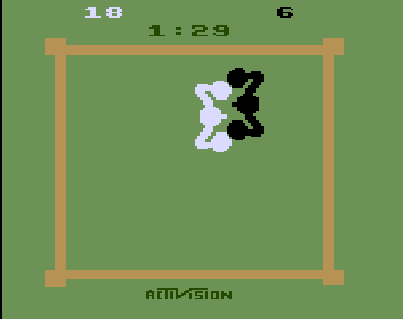
\includegraphics[width=0.7\textwidth]{Figures/boxing}
	\caption{Juego Boxing.}
	\label{fig:boxing}
\end{figure}

En este agente hemos tomado una estrategia agresiva, si el rival lanza un puñetazo, lo intentaremos bloquear con nuestros propios puños poniendo a nuestro boxeador exactamente en la misma posición "Y" que el boxeador contrario (una de las features de Boxing es que la colisión de los puños bloquea los golpes). Además, nuestro boxeador nunca se moverá hacia la izquierda, solo se mueve hacia la derecha en posición de ataque intentando posicionarse en la "Y" del rival, como hemos comentado antes. A su vez, basándonos en ciertas tolerancias, se atacará siempre que sea posible. Esta estrategia agresiva funciona una gran mayoría de las veces, además para evitar el determinismo se ha implementado una pequeña aleatoriedad cada vez que recogemos las posiciones del jugador 1 y del jugador 2 de RAM, como bien se puede ver en el ejemplo de la figura \ref{fig:boxingAleatoriedad}.

\begin{figure}[h]
	\centering
	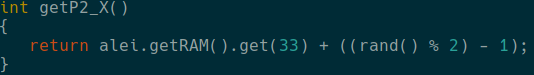
\includegraphics[width=0.7\textwidth]{Figures/BoxingAleatoriedad}
	\caption{Uso de \textbf{rand()} para evitar el determinismo.}
	\label{fig:boxingAleatoriedad}
\end{figure}

A continuación se muestra en el algoritmo \ref{alg:boxingimpl}, la IA implementada. Un detalle a comentar antes de entrar a analizar el algoritmo es que \textbf{player\_pos} es un tipo de dato struct.

%\vspace{2mm}
\begin{algorithm}[H]
	player\_pos p1(getP1\_X(), getP1\_Y())\;
	player\_pos p2(getP2\_X(), getP2\_Y())\;
	absp1p2X := abs(p1.x - p2.x)\;
	absp1p2Y := abs(p1.y - p2.y)\;
	
	\eIf{$absp1p2Y > 3$ \&\& $absp1p2Y < 20$}{
		reward $+= act(FIRE);$
	}{
		\eIf{$absp1p2X > 25$ \&\& $absp1p2X < 40$}{
			reward $+= act(RIGHT);$
		}{
			reward += $(p1.y > p2.y)$ ? act(UP) : act(DOWN)\;
		}
	}
	\caption{Boxing agent}
	\label{alg:boxingimpl}
\end{algorithm}

En la primera parte de recogida de datos, encapsulamos en un struct la posición del jugador uno y la del jugador dos, extrayéndolos de RAM. Como ya hemos comentado anteriormente, estas posiciones implementan una aleatoriedad mínima para evitar ejecuciones deterministas. Además, en la misma sección, calcularemos la distancia entre ambos jugadores en "X" y en "Y", representadas en \textbf{absp1p2X} y \textbf{absp1p2Y} respectivamente, para luego utilizarlas mas adelante.

Una vez tenemos todos los datos procesados, observaremos si nos encontramos en un rango de tolerancia "Y" válido para atacar, si lo estamos, atacaremos (como punto a destacar, este rango es bastante amplio para enfatizar esta estrategia ofensiva). Si no podemos atacar, nos moveremos hacia la derecha  con ciertas tolerancias, o nos situamos en la "Y" del enemigo.


\subsubsection{Demon Attack}
\label{subsec:botsbasicos:da}
El Demon Attack es un juego en el cual controlamos a una nave con un patrón de movimiento similar al Space Invaders. Tendremos que disparar a las naves rivales para pasar de fase además de evitar todo contacto enemigo. El jugador cuenta con una serie de vidas para pasarse los niveles, si estas vidas se acaban el juego termina. De nuevo, vimos la necesidad de crear un bot debido a las bajas puntuaciones obtenidas.

\begin{figure}[h]
	\centering
	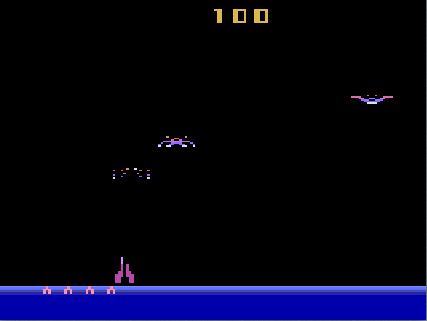
\includegraphics[width=0.9\textwidth]{Figures/demonAttackOne}
	\caption{Juego Demon Attack.}
	\label{fig:demonattackone}
\end{figure}

El Demon Attack es, sin duda, uno de los juegos mas complejos con los que hemos tenido que lidiar, debido a la cantidad de entidades en pantalla, desde disparos hasta múltiples enemigos. La estrategia de IA seguida en el Demon Attack es compleja debido al factor de la gran cantidad de entidades, pues no solo leemos valores en RAM, sino que aprovechamos la característica de \ac{ale} que nos permite leer los píxeles de la pantalla.

Al analizar la RAM, observamos que habían demasiadas características a tener en cuenta, a pesar de tener un análisis detallado de la misma. Hay posiciones de RAM que representan varias cosas en diferentes situaciones, un ejemplo es el valor representado por \textit{RAM[20]}: 

\textit{"20: Coordenada "X" de las balas del enemigo. También es la coordenada "X" de la mosca que se acerca para intentar matar al jugador 1 (se utiliza como una bala). Va desde 29 hasta 147 (incluso cuando dispara la mosca). El valor es todo el rato el mismo hasta que el enemigo dispara y actualiza la coordenada. Si hay mas de 2 cambios consecutivos en 2 frames significa que no es una bala y que es la mosca que sigue al jugador"}.

Es por ello por lo que se dedujo que para implementar un bot básico (sin machine learning), era más fácil hacer un análisis de lo que estuviera pasando en la pantalla en un instante determinado, sin dejar de lado la RAM. Para esto, se diseñó un método de visión en el cual la nave es capaz de ver y filtrar enemigos en un área de visión y actuar concorde la situación dependiendo de unas reglas determinadas. En la figura \ref{fig:demonAttackVision} se puede observar el área de visión de la nave.

\begin{figure}[H]
	\centering
	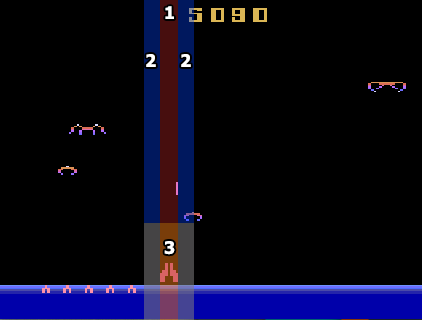
\includegraphics[width=1\textwidth]{Figures/demonAttackVision}
	\caption{Vision de la nave.}
	\label{fig:demonAttackVision}
\end{figure}

La visión de la nave se divide principalmente en 3 partes. En la figura vemos una línea roja representada con el número 1, esta línea roja representa la visión de la nave en función a la anchura de la misma. El número 2 es un área parametrizable que permite ampliar esta visión de forma simétrica por los dos lados de la nave. Tanto el rectángulo rojo como el azul se extienden por casi toda la "Y" de la pantalla y lo único que filtran son los disparos enemigos, como los disparos enemigos tienen el mismo color es muy simple filtrarlos. Por lo tanto 1 y 2 se encargan de detectar disparos enemigos, una vez detectados se actuará en consecuencia.

El número 3 es un área reducida dentro del área completa que se encarga de detectar todas las posibles amenazas, no solo disparos, que estén cerca de la nave. Es decir, el objetivo de la visión es la detección de entidades peligrosas en un área de riesgo para posteriormente evitarlas.

El seguimiento de enemigos para atacarles y matarlos corre a cargo de la RAM, aunque no es del todo exacto debido al problema comentado anteriormente de posiciones de RAM no especificas a una única funcionalidad.

Para analizar la parte práctica de éste algoritmo es necesario separarlo en distintas partes, detección, esquiva y seguimiento.

La parte de detección funciona recogiendo la pantalla entera en grayscale, esto lo hacemos gracias a una funcionalidad de \ac{ale}, una vez tenemos la pantalla guardada, podemos ver cual es el valor de cada píxel. Gracias a esto, podemos determinar el color de los disparos y de las naves enemigas, los que guardaremos en las siguientes variables para después su posterior filtrado:

\begin{figure}[h]
	\centering
	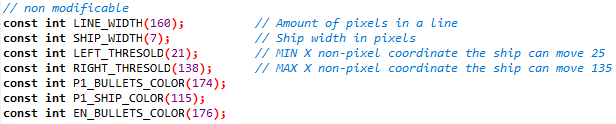
\includegraphics[width=1\textwidth]{Figures/demonAttackStaticOne}
	\caption{Constantes fijas relativas a la visión de la nave.}
	\label{fig:demonAttackStaticOne}
\end{figure}

En la figura \ref{fig:demonAttackStaticOne} podemos observar diversas constantes, entre ellas el color de las balas del jugador 1, \textbf{P1\_BULLETS\_COLOR}, el color de la nave del jugador 1, \textbf{P1\_SHIP\_COLOR} y el color de las balas enemigas, \textbf{EN\_BULLETS\_COLOR}. Gracias a estar en grayscale, con tener un solo valor es suficiente. Además podemos observar otras constantes como \textbf{LINE\_WIDTH}, que representa el ancho en píxeles de la resolución de la Atari, \textbf{SHIP\_WIDTH}, el ancho en píxeles de la nave y \textbf{LEFT / RIGHT\_-THRESOLD}, que es la coordenada "X" mínima y máxima en la que se puede mover la nave aliada.

Además de estas constantes, Demon Attack cuenta con cuatro constantes adicionales que nos permiten parametrizar algunas características de nuestro algoritmo, como se puede ver en la figura \ref{fig:demonAttackChangableOne} .

\begin{figure}[h]
	\centering
	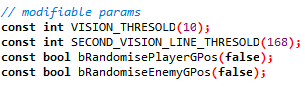
\includegraphics[width=0.7\textwidth]{Figures/demonAttackChangableOne}
	\caption{Constantes modificables (no runtime).}
	\label{fig:demonAttackChangableOne}
\end{figure}

La primera variable de la figura representa el área extra de visión 2 definida en la imagen \ref{fig:demonAttackVision}, la segunda variable define en que línea empieza el área de visión 3. Las dos variables restantes es aleatoriedad opcional a la hora de recoger las posiciones, como se ha hecho antes en el \textit{Boxing}. En este caso, debido a la gran cantidad de entidades en pantalla se ha optado por deshabilitar la aleatoriedad y hacer las batallas mas deterministas.

Otro dato a remarcar antes de empezar con el algoritmo es el Enum utilizado para las colisiones:

\vspace{4mm}
\begin{algorithm}[H]
	enum BlockingHit \{
		$EMoveRight,$
		$EMoveLeft,$
		$ENotBlocking$
	\};
	\caption{Enum empleado para las colisiones.}
	\label{alg:enumcoli}
\end{algorithm}

\vspace{4mm}
Para entender el Enum del algoritmo \ref{alg:enumcoli} tenemos primero que comprender las respuestas que puede dar una colisión y como se operan. 

\begin{itemize}
	\item \textbf{EMoveRight}: La amenaza se ha detectado en la parte izquierda de nuestra área de visión, para contrarrestarla nos moveremos a la derecha si podemos.
	\item \textbf{EMoveLeft}: La amenaza se ha detectado en la parte derecha de nuestra área de visión, para contrarrestarla nos moveremos a la izquierda si podemos.
	\item \textbf{ENotBlocking}: No se ha detectado amenaza ninguna.
\end{itemize}

\newpage
Una vez que ya sabemos qué indicadores utilizaremos para las colisiones, podemos proceder a despiezar el algoritmo.

\begin{figure}[h]
	\centering
	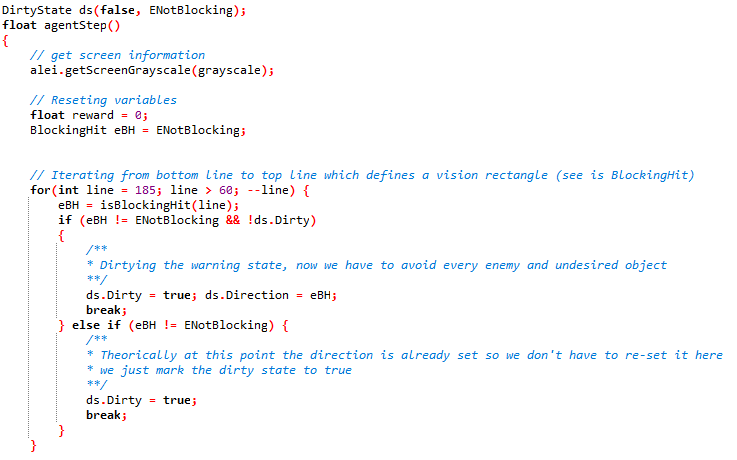
\includegraphics[width=1\textwidth]{Figures/demonattackp1algo}
	\caption{Primera parte del algoritmo de IA para el Demon Attack.}
	\label{fig:demonattackp1algo}
\end{figure}

En esta primera parte recogemos los píxeles de la pantalla con la funcionalidad de \ac{ale} \textbf{getScreenGrayscale}, para luego emplearlos dentro del bucle en la función \textbf{isBlockingHit(int)}, que analizaremos mas adelante. Este bucle se encarga de recorrer 125 filas de la pantalla. En función a la respuesta de \textbf{isBlockingHit(int)}, marcará una variable a true, la cual representa que ha habido una colisión, además dentro de este struct \textbf{DirtyState}, disponemos de otra variable de tipo EBlockingHit para marcar también la dirección contraria a la colisión dada por isBlockingHit. Se ha decidido este thresold ya que el resto de líneas de pantalla contienen información no relevante para el problema.

Para resumir esta parte del código, marcamos el estado a Dirty y recogemos la dirección conveniente, siempre que isBlockingHit haya detectado una colisión. Hasta que no salimos del estado Dirty, no podremos recoger nuevas direcciones, pero de ello se encargará otra parte del código. Es decir, teóricamente se ha implementado una mini máquina de estados finita (FSM), ya que la nave posee dos estados principales (dirty y no dirty) y la forma de transicionar entre ellos es mediante el código de colisiones.

\newpage
\begin{figure}[h]
	\centering
	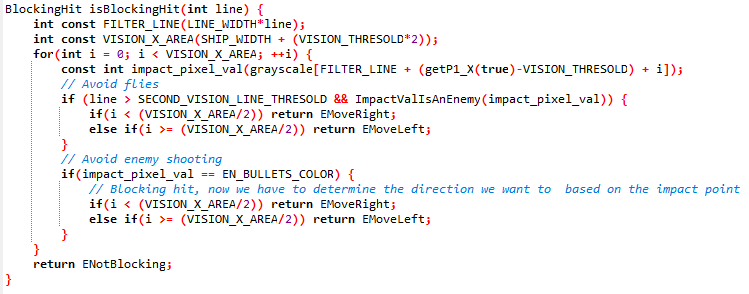
\includegraphics[width=1\textwidth]{Figures/daisblocking}
	\caption{Función isBlockingHit.}
	\label{fig:daisblocking}
\end{figure}

La función isBlockingHit tiene que ser capaz de recorrer el array obtenido por \textbf{getScreenGrayscale} de manera eficiente. Para ello lo primero que hace es resolver la posición del array que ocupa el primer píxel de la línea a analizar, esto es fácil, pues simplemente multiplicando el ancho de la línea con el número de línea ya tenemos este número (asumiendo que las líneas empiezan en 0).

La siguiente tarea es resolucionar el thresold, el cual consiste en el área que ocupa la nave, en este caso 7, mas el thresold determinado, que en nuestro caso corresponde al número de píxeles extras que tendremos en cuenta en cada lado, por ejemplo, si el thresold es 2, el área total será 7+2+2 = 11.

La iteración que haremos en el bucle irá desde 0 hasta el área total que ocupa la visión de la nave, esto es, como ya hemos dicho anteriormente, el área de la nave mas el thresold. Esto hace que solo iteremos los píxeles necesarios para nuestra situación.

La primera línea que encontramos en el bucle puede parecer confusa, pero tiene su explicación:

\vspace{2mm}
\begin{algorithm}[H]
    const int impact\_pixel\_val(grayscale[FILTER\_LINE + (getP1\_X(true)-VISION\_THRESOLD) + i]);
	\caption{Calculo del valor del píxel en un punto determinado de nuestra area de visión.}
	\label{alg:weirdlineda}
\end{algorithm}
\vspace{2mm}

Necesitamos el valor del píxel en un punto determinado de nuestra área de visión. Para ello, necesitamos pedirle al array grayscale esta información, pero antes necesitamos calcular qué posición del array es la correcta. Al haber pre-calculado la posición del array del primer píxel de la línea lo tenemos mucho mas fácil, pues tenemos por donde empezar. A ese número le tenemos que sumar la posición del jugador uno, representado en \textbf{getP1\_X(true)}, al cual le pasamos el parámetro true para que nos devuelva la posición en píxeles, la cual es más precisa para este problema. Una vez tenemos la posición del jugador solo nos queda sumarle i para abordar todo el área de visión. Pero como bien podemos observar en el algoritmo \ref{alg:weirdlineda}, estamos restando a la posición del jugador el \textbf{VISION\_THRESOLD}, esto se hace porque sino estaríamos solo teniendo en cuenta el área extra por la derecha, ya que la colisión estaría desplazada a la izquierda como muestra la figura 	\ref{fig:colisioncalculadaerroneamenteda}, por ello es necesario restar \textbf{VISION\_THRESOLD}.,

\begin{figure}[h]
	\centering
	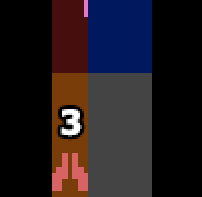
\includegraphics[width=0.3\textwidth]{Figures/colisioncalculadaerroneamenteda}
	\caption{Area de sin restar VISION\_THRESOLD al jugador.}
	\label{fig:colisioncalculadaerroneamenteda}
\end{figure}

Una vez hemos resolucionado el valor del píxel, podemos hacer el filtrado del mismo, el cual se realizará en el cuerpo del bucle.

\begin{figure}[h]
	\centering
	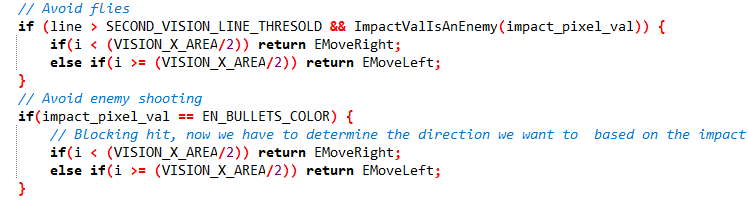
\includegraphics[width=1\textwidth]{Figures/cuerpobucleisblockingda}
	\caption{Resolución de la colisión}
	\label{fig:cuerpobucleisblockingda}
\end{figure}

Como bien observamos en la figura 	\ref{fig:cuerpobucleisblockingda}, haremos una primera distinción para las moscas y enemigos mas cercanos a nuestra segunda área de visión seguido de la visión normal. Priorizamos el segundo área de visión porque está mas cerca del jugador, lo cual se traduce en más peligro a perder una vida. En el primer if, miramos si nos encontramos en el área de riesgo y filtramos por color principalmente si lo que hay en ese píxel es un enemigo. Si es así, es que ha habido una colisión. Si la i en la cual nos encontramos es menor (o está a la izquierda) de la mitad del área de visión, nos moveremos a la derecha (camino más corto para evitar la colisión). Haremos lo mismo para el otro ladro. El segundo if es exactamente lo mismo solo que nos centramos únicamente en las balas enemigas.

Finalmente, si no se ha encontrado colisión ninguna, como hemos visto en la figura \ref{fig:daisblocking}, devolveremos \textit{ENotBlocking}.

\begin{figure}[h]
	\centering
	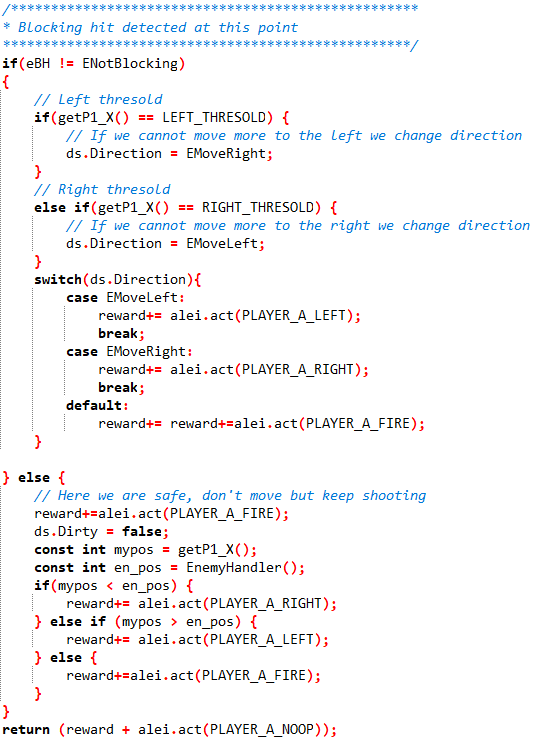
\includegraphics[width=0.76\textwidth]{Figures/damovement}
	\caption{Aplicando movimiento a la nave}
	\label{fig:damovement}
\end{figure}

La parte que extiende a la figura \ref{fig:demonattackp1algo}, es la figura \ref{fig:damovement}. En ésta figura podemos observar la parte del algoritmo que finalmente aplica movimiento a la nave. En este punto ya hemos solucionado la colisión y solo nos queda movernos en la dirección conveniente.

Esta parte del código se divide en dos dependiendo respectivamente si hemos encontrado una colisión o no. En la primera parte ya tenemos en el \textbf{DirtyState} apuntado la dirección en la cual movernos, sin embargo si nos encontramos en los bordes de la pantalla, no nos podremos mover la la dirección del borde, es por esto por lo que cambiamos de dirección cuando llegamos a un borde. Si no estamos en ningún borde, simplemente aplicamos la dirección anotada por \textbf{ds.Direction}.

\begin{figure}[h]
	\centering
	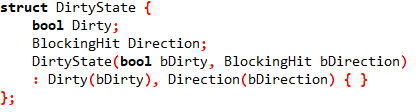
\includegraphics[width=0.79\textwidth]{Figures/structdirtystateda}
	\caption{Struct Dirty State}
	\label{fig:structdirtystateda}
\end{figure}

En la segunda parte, podemos considerar que el jugador uno está a salvo de posibles ataques enemigos, esto viene determinado, como ya hemos comentado anteriormente, por el resultado de isBlockingHit. Por lo tanto, lo que haremos en este modo es disparar siempre que podamos a la vez que intentar traquear a los enemigos en RAM para dispararles dentro de su colisión. \textbf{EnemeyHandler} se encargará de devolvernos el enemigo mas relevante en un instante determinado (usualmente el mas cercano al jugador). Esta función no funciona el 100\% de los casos, ya que como hemos comentado anteriormente, la RAM no es específica a casos concretos sino que va cambiando, por lo tanto habrá, veces que el jugador 1 se quede disparando a la nada porque no tiene nada que trackear. Esto se resuelve parcialmente gracias a la aleatoriedad y al movimiento de las entidades enemigas, que acabaremos matando si se acercan a nuestro láser. La solución completa y real sería llevar un seguimiento mas especifico de todas las unidades en RAM, lo cual puede llevarnos a implementar demasiados casos específicos para un escenario mas simple de solucionar mediante un algoritmo genérico (mediante una buena función de fitness) o un neuroevolutivo en su defecto.


%----------------------------------------------------------------------------------------------%
%----------------------------------------------------------------------------------------------%
%----------------------------------------------------------------------------------------------%
%----------------------------------------------------------------------------------------------%
\newpage
\subsection{Perceptrón}
\label{subsec:perceptron}

El perceptrón es una de las técnicas de \textit{Machine Learning} más sencillas de comprender, implementar y útiles. En su sencillez radica los buenos resultados que suele dar, siempre que el problema a resolver no sea muy complejo, ya que pasado cierto nivel de complejidad, el perceptrón seguramente no sea la mejor opción. El perceptrón lo que intenta hacer es separar los datos que le demos, asegurándonos que obtendrá la mejor solución posible si los datos de los cuales partimos son linealmente separables, y en el caso de no serlo, deberemos dar la mejor solución posible (aquella con menor error).

El perceptrón es una técnica de aprendizaje supervisado en la que le damos datos etiquetados y, a partir del error obtenido al intentar etiquetar los datos, se hacen ajustes en la configuración para acercarnos más a los resultados correctos. Esta técnica puede utilizarse para clasificación o para regresión. El resultado que al final obtendremos será, dependiendo del número de entradas que tengamos, una línea, un plano o un hiperplano. Los elementos del perceptrón son las entradas, los pesos y la salida.

\begin{figure}[h]
    \centering
    
    \tikzset{basic/.style={draw,fill=blue!20,text width=1em,text badly centered}}
    \tikzset{input/.style={basic,circle}}
    \tikzset{weights/.style={basic,rectangle}}
    \tikzset{functions/.style={basic,circle,fill=blue!10}}
    
    \begin{tikzpicture}
        \node[] (center) {};
        \node[functions,left=3em of center] (left) {$\sum$};
            \path[draw,->] (left) -- (center);
        \node[weights,left=3em of left] (2) {$w_3$} -- (2) node[input,left of=2] (l2) {$x_3$};
            \path[draw,->] (l2) -- (2);
            \path[draw,->] (2) -- (left);
        \node[below of=2] (dots) {$\vdots$} -- (dots) node[left of=dots] (ldots) {$\vdots$};
        \node[weights,below of=dots] (n) {$w_n$} -- (n) node[input,left of=n] (ln) {$x_n$};
            \path[draw,->] (ln) -- (n);
            \path[draw,->] (n) -- (left);
        \node[weights,above of=2] (1) {$w_2$} -- (1) node[input,left of=1] (l1) {$x_2$};
            \path[draw,->] (l1) -- (1);
            \path[draw,->] (1) -- (left);
        \node[weights,above of=1] (0) {$w_1$} -- (0) node[input,left of=0] (l0) {$x_1$};
            \path[draw,->] (l0) -- (0);
            \path[draw,->] (0) -- (left);
        \node[below of=ln,font=\scriptsize] {inputs};
        \node[below of=n,font=\scriptsize] {weights};
        \node[right of=center,font=\scriptsize] {output};
    \end{tikzpicture}
    
    \caption{Estructura básica del perceptrón}
    \label{fig:perceptron}
\end{figure}

La salida que tiene el perceptrón, en el caso del clasificador, es siempre de +1 o -1. Para obtener esta salida, la fórmula que se aplica es la siguiente cuando tenemos N entradas:

\[y=signo(\sum_{i=1}^{N}x_{i}*w_{i})\]

Ahora bien, como hemos dicho, lo que el perceptron hace es separar datos, es decir, encontrar la linea, plano o hiperplano que los separa, pero si nos fijamos en la fórmula que hemos descrito encontramos un problema, y es que no hay término independiente, todos los pesos están asociados con alguna entrada, por lo que la linea, plano o hiperplano siempre pasará por el origen de coordenadas, cosa que seguramente no sea así para la mayoría de los problemas. La solución es, como hemos dicho, añadir un término independiente, al cual se le suele llamar \textit{bias}. Una manera de hacerlo es añadir un peso w0 y una entrada x0 artificial que siempre tenga el valor 1, con lo que al final nos queda la siguiente fórmula:

\[x_0=1\]
\[y=signo(\sum_{i=0}^{N}x_{i}*w_{i})\]

Finalmente, la figura \ref{fig:completeperceptron} muestra la estructura final del perceptrón.

\begin{figure}[h]
    \centering
    
    \tikzset{basic/.style={draw,fill=blue!20,text width=1em,text badly centered}}
    \tikzset{input/.style={basic,circle}}
    \tikzset{weights/.style={basic,rectangle}}
    \tikzset{functions/.style={basic,circle,fill=blue!10}}
    
    \begin{tikzpicture}
        \node[functions] (center) {};
        \node[below of=center,font=\scriptsize,text width=3em,align=center] {sign function};
        \draw[thick] (0.5em,0.5em) -- (0,0.5em) -- (0,-0.5em) -- (-0.5em,-0.5em);
        \draw (0em,0.75em) -- (0em,-0.75em);
        \draw (0.75em,0em) -- (-0.75em,0em);
        
        \node[functions,left=3em of center] (left) {$\sum$};
            \path[draw,->] (left) -- (center);
        \node[weights,left=3em of left] (2) {$w_2$} -- (2) node[input,left of=2] (l2) {$x_2$};
            \path[draw,->] (l2) -- (2);
            \path[draw,->] (2) -- (left);
        \node[below of=2] (dots) {$\vdots$} -- (dots) node[left of=dots] (ldots) {$\vdots$};
        \node[weights,below of=dots] (n) {$w_n$} -- (n) node[input,left of=n] (ln) {$x_n$};
            \path[draw,->] (ln) -- (n);
            \path[draw,->] (n) -- (left);
        \node[weights,above of=2] (1) {$w_1$} -- (1) node[input,left of=1] (l1) {$x_1$};
            \path[draw,->] (l1) -- (1);
            \path[draw,->] (1) -- (left);
        \node[weights,above of=1] (0) {$w_0$} -- (0) node[input,left of=0] (l0) {$1$};
            \path[draw,->] (l0) -- (0);
            \path[draw,->] (0) -- (left);
        \node[below of=ln,font=\scriptsize] {inputs};
        \node[below of=n,font=\scriptsize] {weights};
        \node[right of=center,font=\scriptsize] {output};
    \end{tikzpicture}
    
    \caption{Estructura del perceptrón}
    \label{fig:completeperceptron}
\end{figure}

En nuestro trabajo hemos implementado el algoritmo de aprendizaje del perceptrón (PLA), el cual nos permite ir ajustando la configuración del perceptrón, lo que quiere decir que vamos ajustando los pesos con el fin de que obtengamos el resultado que buscamos para las entradas. El algoritmo de aprendizaje del perceptrón se muestra en el algoritmo \ref{alg:pla}.

\vspace{2mm}
\begin{algorithm}[H]
    predictions $= getPredictions(inputs);$
    
    mPoint $= getRandomMisclassfiedPoint(predictions, targets);$
    
    \eIf{$mPoint.empty()$}
    {
		$return;$
	}
	{
	    \For{$i \gets 0$ to $N$}
        {
            weights[i] $+= mPoint.target$*$mPoint.prediction$
        }
	}
	\caption{PLA}
	\label{alg:pla}
\end{algorithm}
\vspace{2mm}

El código del PLA debería ejecutarse tantas veces como fuera necesario, y eventualmente llegaría a una solución, siempre que los datos fueran linealmente separables. Ya que no siempre van a ser linealmente separables, podemos poner un bucle y hacer tantas iteraciones como fuera necesario (a cada iteración de este bucle se le conoce con el concepto de \textbf{época}).

\vspace{2mm}
\begin{algorithm}[H]
    \For{$epoch \gets 1$ to $epochs$}
    {
        predictions $= getPredictions(inputs);$
        
        mPoint $= getRandomMisclassfiedPoint(predictions, targets);$
        
        \eIf{$mPoint.empty()$}
        {
    		$return;$
    	}
    	{
    	    \For{$i \gets 0$ to $N$}
            {
                weights[i] $+= mPoint.target$*$mPoint.prediction$
            }
    	}
	}
	\caption{PLA con épocas}
	\label{alg:plawithepochs}
\end{algorithm}
\vspace{2mm}

Por último, vemos el problema de que si no tenemos datos linealmente separables, las épocas no solucionan el problema totalmente (solucionan el problema de no quedarnos en un bucle infinito), ya que puede que antes de llegar a la última época, ya hayamos encontrado una solución bastante buena, pero que la hayamos perdido por el camino al actualizar los pesos, por lo que a cada época que se esté ejecutando el PLA, deberíamos de estar guardando la mejor solución hasta el momento. A esto se le conoce con el nombre del algoritmo \textit{Pocket}.

\newpage
\begin{algorithm}[H]
    pocket $= []$
    
    \For{$epoch \gets 1$ to $epochs$}
    {
        predictions $= getPredictions(inputs);$
        
        mPoint $= getRandomMisclassfiedPoint(predictions, targets);$
        
        \If{$numberOfMisclassifiedPoints(pocket, targets)$ > $numberOfMisclassifiedPoints(weights, targets)$}
        {
            pocket $= weights$
        }
        
        \eIf{$mPoint.empty()$}
        {
    		$return;$
    	}
    	{
    	    \For{$i \gets 0$ to $N$}
            {
                weights[i] $+= mPoint.target$*$mPoint.prediction$
            }
    	}
	}
	
	\If{$!pocket.empty()$}
	{
	    weights $= pocket$
	}
	\caption{PLA con épocas y Pocket}
	\label{alg:plawithepochsandpocket}
\end{algorithm}
\vspace{2mm}

Nuestro código es muy similar al descrito, ya que la parte más importante es la que hemos explicado, la del PLA. La estructura que hemos empleado es la de una clase llamada \textbf{Perceptron} que contiene los métodos necesarios para obtener una predicción, la cual se obtiene haciendo uso del método \textit{double getPrediction(const vector\textless double\textgreater \&inputs)} y el PLA se ejecuta haciendo uso del método \textit{void trainPerceptron(unsigned epochs, const vector\textless vector\textless double\textgreater \textgreater \&inputs, const vector\textless double\textgreater \&targets)}.

\newpage
\subsection{Redes neuronales}
\label{subsec:nn}


\newpage
\subsubsection{Algoritmo Genético (GANN)}
\label{subsubsec:nn:gann}

Los algoritmos genéticos pertenecen a la categoría de los algoritmos evolutivos, los cuales intentan optimizar algún problema basándose en la biología, basándose en como la naturaleza ha evolucionado a lo largo de miles de años e intentando utilizar la misma técnica. Concretamente, los algoritmos genéticos intentan imitar la estructura genética de los individuos y como esta estructura va evolucionando de una generación de individuos a la siguiente, esa es la idea principal de dichos algoritmos. Antes de pasar a explicar la combinación de los algoritmos genéticos con las redes neuronales vamos a explicar las ideas principales de los algoritmos genéticos.

Como hemos dicho, los algoritmos genéticos se basan en la evolución de la estructura genética de los individuos y como se transmite esta herencia genética de una generación a la siguiente. Hablando sobre esta estructura, todo \textbf{individuo} vivo tiene una serie de \textbf{células} y cada una de estas células contiene el mismo conjunto de \textbf{cadenas de ADN}, lo que se conoce como \textbf{cromosomas}. El ADN que contiene un cromosoma es una doble cadena en forma de hebra, y las hebras están conectadas entre sí en una \textbf{doble espiral}. Finalmente, esta doble espiral está formada por pequeños bloques básicos, llamados \textbf{genes}, que a su vez están formados por sustancias llamadas \textbf{nucleótidos}. Solo hay 4 tipos de nucleótidos: timina, adenina, guanina y citosina. En la figura \ref{fig:basicDNAStructure} se puede apreciar lo que hemos comentado de una manera más gráfica. Esta es la estructura básica de la información genética de los seres vivos.

Ahora sabemos un poco más cuál es la estructura básica, pero aún no hemos explicado qué es lo que contienen estas partes, lo cual va a ser lo importante para poder comprender correctamente el funcionamiento biológico y así poder hacer una buena aproximación con los algoritmos genéticos a este enfoque de la evolución respecto a la herencia genética. Lo importante es comprender que la información que hay dentro de una célula (conjunto de cadenas de ADN, los cromosomas) es lo que contiene toda la información que define a un individuo y, por lo tanto, tiene toda la información que podría pasarse al individuo de la siguiente generación (normalmente de forma parcial, no total). Esta colección de cromosomas (información genética dentro de la célula) es lo que se conoce como \textbf{genoma}, que no es más que la colección de genes que definen las características del individuo (e.g. ojos marrones, pelo liso, color del pelo, etc.). Volviendo a los \textbf{genes}, la configuración que cada gen puede tener es lo que da rasgo a alguna característica concreta, y a esto se le llama \textbf{alelo} (característica concreta del individuo), y la posición física donde está el gen a lo largo de la cadena del cromosoma se le llama \textbf{locus}.

\begin{figure}[h]
	\centering
	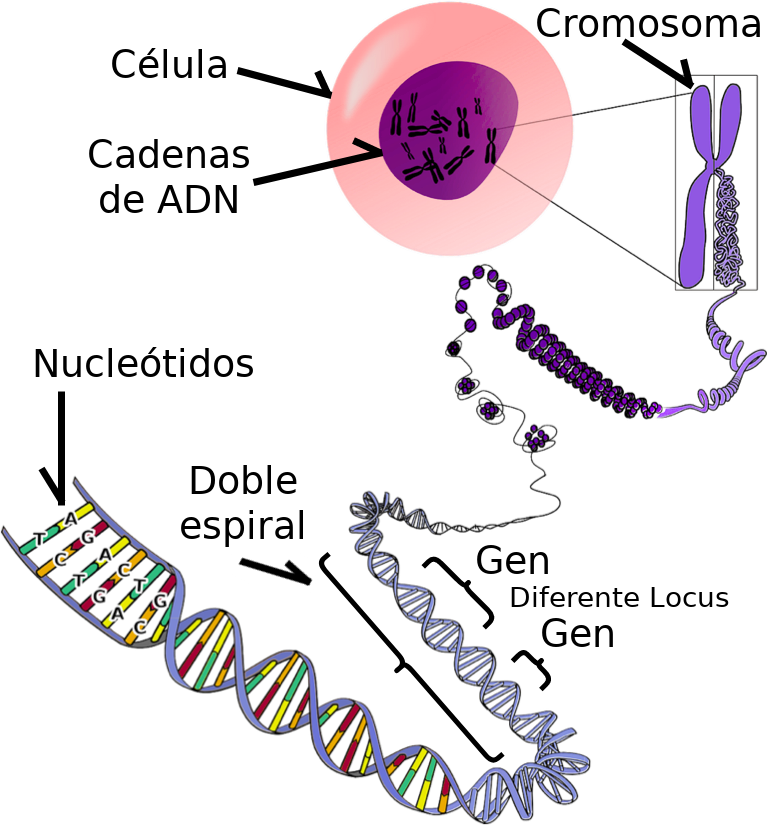
\includegraphics[width=0.79\textwidth]{Figures/basicDNAStructure}
	\caption{Estructura básica del ADN}
	\label{fig:basicDNAStructure}
\end{figure}

Ahora bien, el estado de los alelos en un genoma particular se conoce como \textbf{genotipo} (información genética que da lugar a las características del individuo). El genotipo es una información que una vez está definida no cambia. Al organismo en sí, al individuo, a la expresión de ese genotipo en el mundo real, se le conoce como \textbf{fenotipo}. Por poner un ejemplo, el ADN que tiene cada ser humano sería el genotipo propio de cada uno, mientras que la persona en sí, el como se expresa en el mundo físico, sería su fenotipo, el cual, además, está influido por el ambiente. En la figura \ref{fig:genotypeVSphenotype} se ve esta diferencia claramente, que es lo que se conoce como genotipo vs fenotipo.

\begin{figure}[h]
    \centering
    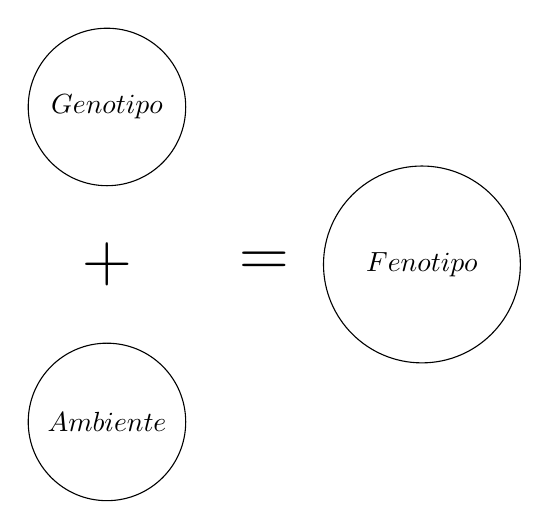
\begin{tikzpicture}
        %\draw (0,0) grid (3,3);
        %\draw (0,0) circle [radius=0.3] node {$Genotipo$};
        \node[draw,circle,minimum size=2cm,inner sep=0pt] at (0,0) {$Genotipo$};
        \node[draw,circle,minimum size=2.5cm,inner sep=0pt] at (4,-2) {$Fenotipo$};
        \node[draw,circle,minimum size=2cm,inner sep=0pt] at (0,-4) {$Ambiente$};
        \node[draw=none,fill=none,font=\fontsize{1cm}{1cm}\selectfont] at (0,-2) {$+$};
        \node[draw=none,fill=none,font=\fontsize{1cm}{1cm}\selectfont] at (2,-2) {$=$};
    \end{tikzpicture}
    \caption{Genotipo vs Fenotipo}
	\label{fig:genotypeVSphenotype}
\end{figure}

Observando la figura \ref{fig:genotypeVSphenotype}, podemos darnos cuenta de algo, y es que aunque tengamos 2 copias exactas a nivel genético de un individuo (i.e. clones), lo que significaría que tienen el mismo genotipo, podrían no tener el mismo fenotipo, ya que el ambiente importa, aunque respecto a los algoritmos genéticos esto se obvía normalmente, al no ser que de alguna forma el individuo evolucione mientras está en vida (nos referimos a algoritmos, no a seres vivos). Si tuviéramos un algoritmo genético que combinado con otra técnica, el individuo evolucionase a la vez que se ejecuta entonces podríamos hablar de que el entorno importa (e.g. algoritmo genético que resuelve un camino en un laberinto y aprende a la vez que lo recorre, pero además el laberinto varía, por lo que un individuo podría aprender muy bien a resolverlo, pero otro individuo con el mismo genotipo tiene un laberinto complicado, por lo que no aprende bien, así que el fenotipo varía).

Una vez hablado de todo lo anterior, lo que es la parte biológica, necesario para comprender correctamente el funcionamiento de un algoritmo genético, podemos pasar a explicar como funciona el algoritmo en sí. Los algoritmos genéticos lo que intentan es aproximar el enfoque de la evolución desde el punto de vista de la herencia genética: de algún modo codifican el genotipo del individuo, de algún modo se evalúa lo bien que hace su tarea para sobrevivir, para tener más posibilidades de pasar parte de su información genética a la siguiente generación, y se hace evaluando su fenotipo. En definitiva, los algoritmos genéticos se basan en los principios de Charles Darwin de su teoría de la selección natural. Resumidamente es la supervivencia del más apto.

Las fases principales de los algoritmos genéticos son:
\begin{enumerate}
    \item Crear una \textbf{población inicial} de individuos. Esta población suele generarse de forma aleatoria y, aunque muchos individuos harán mal su tarea, otros lo harán medio bien o incluso bien. También se pueden inicializar siguiendo una distribución de probabilidad que se sabe que sigue el patrón de los individuos que hacen bien su tarea.
    \item Calcular su \textbf{\textit{fitness}}. Este valor se calcula de la función de \textit{fitness}, la cual nos indica como de bien un individuo hace la tarea para la que se supone que ha sido concebido. El objetivo suele ser maximizar esta función.
    \item \textbf{Selección}. Seleccionar los individuos más aptos para pasar su información a la siguiente generación. Esto es una cuestión de probabilidad, no de directamente hacer que los mejores individuos sean los que pasen su información a la siguiente generación. Los mejores individuos tendrán más posibilidades, pero los peores también tendrán una pequeña posbilidad de pasar su información a la siguiente generación.
    \item \textbf{\textit{Crossover} (emparejamiento)}. Unir la información genética de los individuos seleccionados para pasar a la siguiente generación.
    \item \textbf{Mutación}. Las mutaciones son algo que sucede cuando hablamos de la genética. A veces son buenas y a veces son malas, pero está claro que son necesarias. La mutación puede aportarnos algo que puede que ningún individuo de la población inicial tuviera en su información genética, y esa mutación podría hacer que un nuevo gen surgiera y predominara por encima de todos.
    \label{enum:geneticAlgorithmSteps}
\end{enumerate}

La estructura principal de los algoritmos genéticos se muestra en el algoritmo \ref{alg:generalGAStructure}.

\vspace{2mm}
\begin{algorithm}[H]
    population $= createNewPopulation();$
    
    \While{true}
    {
        fitness $= evaluatePopulation(population);$
        
        newPopulation $= [];$
        
        \For{$individual \gets 1$ to $population$}
        {
            parents $= doSelection(population, fitness);$
            
            newIndividual $= doCrossover(parents);$
            
            newIndividual $= doMutation(newIndividual);$
            
            newPopulation[individual] $= newIndividual;$
        }
        
        population $= newPopulation;$
    }
	\caption{Estructura general de los algoritmos genéticos}
	\label{alg:generalGAStructure}
\end{algorithm}
\vspace{2mm}

Conforme se vaya pasando de generación en generación, los nuevos individuos irán mejorando, ya que han ido obteniendo los mejores genes de sus antepasados o al menos esa es la idea principal de estos algoritmos. Dentro de estos algoritmos luego hay muchos aspectos que controlar para que estos funcione como es debido, aunque lo básico ya está expuesto. Ahora pasaremos a hablar por qué pueden ser útiles a la hora de combinarlos con las redes neuronales.

Las redes neuronales forman parte de los algoritmos de aprendizaje supervisado, lo que quiere decir que necesita de datos que previamente estén etiquetados. Con estos datos utiliza el algoritmo de aprendizaje \textit{back propagation} (propagación hacia atrás), el cual es el mejor algoritmo de aprendizaje hasta la fecha para las redes neuronales para el aprendizaje supervisado, pero no el único. La idea de juntar los algoritmos genéticos con las redes neuronales (GANN) es la de no utilizar el algoritmo de aprendizaje \textit{back propagation}, sino que en su lugar utilizar el propio algoritmo genético como algoritmo de aprendizaje para la red neuronal. Como hemos dicho, el algoritmo de aprendizaje \textit{back propagation} es el mejor que se conoce a día de hoy para el aprendizaje supervisado en las redes neuronales, así que ¿cuál es el objetivo de utilizar un algoritmo genético como algoritmo de aprendizaje? Hay varias razones, y una de las principales razones es que al utilizar un algoritmo genético como algoritmo de aprendizaje para las redes neuronales dejamos de estar utilizando aprendizaje supervisado y pasamos a estar utilizando \textbf{aprendizaje por refuerzo}.

El aprendizaje por refuerzo no necesita de datos etiquetados como sí lo necesita el aprendizaje supervisado. Este en su lugar necesita una medida de como de bien está comportándose el algoritmo, lo cual encaja a la perfección con la función de \textit{fitness}, que es justamente lo que hace. La idea es codificar de alguna manera las redes neuronales de manera que un algoritmo genético pueda tratarlas, modificarlas, etc. Tenemos que conseguir el genotipo de la red neuronal, y la forma de hacerlo es con la codificación de la red. Hay muchos tipos de codificaciones, siendo la más típica la \textbf{codificación binaria}, la cual coge \textit{N} bits para representar un peso de la red neuronal y entonces ya ejecuta todas las fases que hemos comentado. Esta codificación es la más típica, pero también es muy restrictiva y nos aporta poca flexibilidad. En nuestro caso, la codificación que hemos hecho de la red neuronal es una codificación de \textbf{números reales}, en la cual cada peso de la red se trata como lo que es, un número real. Esta codificación también trae problemas, siendo uno de ellos el límite superior e inferior que se le da a los pesos, ya que en función de esos límites podremos generar unos pesos en un rango o en otro.

Por la forma en la que tenemos nuestra implementación de la red neuronal, en la cual hemos implementado el perceptrón multicapa, la manera más sencilla para representar la red, para codificarla, era coger nuestras matrices de pesos y aplanarlas para obtener un vector. Respecto a los \textit{biases} hicimos lo mismo, coger la matriz que contiene todos los \textit{biases}, aplanarla, y añadir todos los pesos al final del vector que contiene los pesos. Como luego es necesario decodificar y volver a obtener nuestras matrices de pesos y \textit{biases}, con el vector de topología, que es el vector que nos indica cual es la topología de esa codificación en concreto, se puede volver a desaplanar sin ningún problema. El aplanamiento y unión de matrices de pesos y \textit{biases} es sencillo, pero el desaplanar puede no serlo tanto, así que se puede observar el código en el algoritmo \ref{alg:unflatteningOfWeightsAndBiases}.

\vspace{2mm}
\begin{algorithm}[H]
\KwData{const vector\textless int\textgreater \&topology, const Mat \&flattened}
\KwResult{vector\textless vector\textless Mat\textgreater\textgreater weightsAndBiases}
    $vector$\textless $vector$\textless $Mat$\textgreater\textgreater $res;$
    
    $vector$\textless $Mat$\textgreater $weights;$
    
    $vector$\textless $Mat$\textgreater $bias;$
    
    $int$ $flattenedCol = 0;$
    
    \For{$(size\_t$ $i = 0; i < topology.size() - 1; i++)$}
    {
        $Mat$ $matWeights(topology[i], topology[i + 1]);$

        \For{$(int$ $row = 0; row < matWeights.rows(); row++)$}
        {
            \For{$(int$ $col = 0; col < matWeights.cols(); col++)$}
            {
                $matWeights.set(row, col, flattened.get(0, flattenedCol));$

                $flattenedCol++;$
            }
        }

        $weights.push\_back(matWeights);$
    }
    \For{$(size\_t$ $i = 0; i < topology.size() - 1; i++)$}
    {
        $Mat$ $matBias(1, topology[i + 1]);$

        \For{$(int$ $col = 0; col < matBias.cols(); col++)$}
        {
            $matBias.set(0, col, flattened.get(0, flattenedCol));$

            $flattenedCol++;$
        }

        $bias.push\_back(matBias);$
    }

    $res.push\_back(weights);$
    $res.push\_back(bias);$

    $return$ $res;$
    
	\caption{Desaplanamiento de las matrices de pesos y \textit{biases}}
	\label{alg:unflatteningOfWeightsAndBiases}
\end{algorithm}
\vspace{2mm}

Una vez ya desaplanados los pesos y \textit{biases} ya solo nos quedaba crear una nueva red neuronal y utilizar \textit{setWeights()} y \textit{setBiases()}.

Ahora vamos a pasar a la parte más importante de nuestra implementación de la GANN, que son los operadores genéticos que hemos empleado. Los operadores genéticos son las operaciones que realizamos para obtener la selección, el emparejamiento y la mutación de los individuos.

Para la selección de los individuos hay varios operadores genéticos, siendo los más famosos los siguientes:

\begin{enumerate}
    \item Selección proporcional del \textit{fitness} (Fitness proportionate selection) más conocido con el nombre de Roulette Wheel Selection. Este operador de selección consiste en asignarle a cada individuo una probabilidad basada en su \textit{fitness} respecto a la suma total del \textit{fitness} de toda la población. De esta manera, luego se simula la rotación de una ruleta, donde los que mayor probabilidad tienen son los que mayor sector tienen en la ruleta. Es el operador de selección más utilizado y \underline{es el que hemos utilizado en nuestra implementación}. La fórmula que utiliza es la siguiente:
    \[p_{i}=\dfrac{f_{i}}{\sum_{j=1}^{N}{f_{j}}}\]
    \item Selección por torneo. Este método intenta simular un torneo, donde la probabilidad de selección varía a cada iteración. Cuando se han ejecutado los torneos que se haya configurado, es cuando se escoge a los mejores individuos (donde K es el número de individuos que participan en el torneo). La fórmula que utiliza es la siguiente:
    \[p_{0}=p\]
    \[p_{iteration}=p*(1-p)^{iteration}\]
    \item Selección basada en recompensas. Este método recomensa a los individuos que han hecho algo de forma correcta. Hay muchas fórmulas que pueden ser utilizadas como recomensa, una básica es la siguiente:
    \[individual^{(generation + 1)} selected \Rightarrow reward^{(generation)} = 1\]
\end{enumerate}

Respecto al emparejamiento de individuos, hay muchas maneras de hacerlo. Nosotros utilizamos 2 enfoques diferentes, y en ambos era para el emparejamiento de 2 individuos, es decir, de 2 redes neuronales. En el primero de ellos lo que hacíamos era alternar entre coger un peso de una red y luego otro de la otra, con lo que acabábamos con una nueva red con cerca del 50\% del genotipo de las 2 redes que se utilizaban como padres. El segundo enfoque lo que hacíamos era coger los 2 pesos de la misma posición de los padres y hacer una media ponderada, lo cual nos daba más seguridad de que los resultados obtenidos en la función de \textit{fitness} de la nueva red neuronal iban a ser más próximos a los de las redes padre, ya que si ambas redes neuronales padre obtenían buenos valores de \textit{fitness} la probabilidad de que sus pesos se parecieran es muy alta, como veremos que sucede en los experimentos realizados. Esta último enfoque es el que se ha quedado en la última versión del GANN. Podemos ver ambos enfoques en el algoritmo \ref{alg:crossoverOperator}.

\begin{algorithm}[H]
\KwData{const DNA \&a, double ownFitness, double aFitness}
\KwResult{DNA newIndividual}
    $DNA$ $res(a.genes.rows(), a.genes.cols());$

    $double$ $random = UtilG::getRandomDouble(0.0, 1.0);$

    \eIf{$random <= this->crossoverRate$}
    {
        $res.setMutationRate(this->mutationRate);$
        
        $res.setCrossoverRate(this->crossoverRate);$

        \If{$a.genes.rows() == this->genes.rows() \&\&
            a.genes.cols() == this->genes.cols()$}
        {
            \For{$(int$ $row = 0; row < a.genes.rows(); row++)$}
            {
                \For{$(int$ $col = 0; col < a.cols(); col++)$}
                {
                    $//$ $First$ $approach$
                    
                    \eIf{$(row + col) \% 2 == 0$}
                    {
                        $res.genes.set(row, col, this->genes.get(row, col));$
                    }
                    {
                        $res.genes.set(row, col, a.genes.get(row, col));$
                    }

                    $//$ $Second$ $and$ $definitive$ $approach.$ $Average$
                    
                    $res.genes.set(row, col, (a.genes.get(row, col) + this->genes.get(row, col)) / 2.0);$
                }
            }
        }
    }
    {
        \eIf{$ownFitness > aFitness$}
        {
            $res = *this;$
        }
        {
            $res = a;$
        }
    }

    $return$ $res;$
    
	\caption{Operadores genéticos de emparejamiento empleados}
	\label{alg:crossoverOperator}
\end{algorithm}

Por último, al igual que con los operadores genéticos de emparejamiento, hay muchas posibilidades para los operadores genéticos de mutación. En nuestra implementación aplicamos 2 tipos de mutaciones. La primera mutación que aplicamos es cambiar un número real por otro, por defecto en el rango [-1.0, 1.0], aunque es posible multiplicar dicho rango por factor, dando lugar a [-1.0*factor,1.0*factor]. El otro operador genético de mutación que hemos empleado ha sido la permutación. La implementación de ambos operadores se muestra en el algoritmo \ref{alg:mutationOperator}.

\vspace{2mm}
\begin{algorithm}[H]
    
    $//$ $First$ $mutation.$ $Replace$ $a$ $real-number$
    
    \For{$(int$ $row = 0; row < this->genes.rows(); row++)$}
    {
        \For{$(int$ $col = 0; col < this->genes.cols(); col++)$}
        {
            $double$ $random = UtilG::getRandomDouble(0.0, 1.0);$

            \If{$random <= this->mutationRate$}
			{
				$this->genes.set(row, col, UtilG::getRandomDouble((double)factor * -1.0, (double)factor * 1.0));$
			}
        }
    }
    
    $//$ $Second$ $mutation.$ $Permute$ $2$ $weights/biases$
    
    \For{$(int$ $row = 0; row < this->genes.rows(); row++)$}
    {
        \For{$(int$ $col = 0; col < this->genes.cols(); col++)$}
        {
            $double$ $random = UtilG::getRandomDouble(0.0, 1.0);$

            \If{$random <= this->mutationRate$}
			{
                $int$ $randomRow1 = rand() \% this->genes.rows();$
                $int$ $randomCol1 = rand() \% this->genes.cols();$
                $int$ $randomRow2 = rand() \% this->genes.rows();$
                $int$ $randomCol2 = rand() \% this->genes.cols();$
                $double$ $value1 = this->genes.get(randomRow1, randomCol1);$
                $double$ $value2 = this->genes.get(randomRow2, randomCol2);$

                $this->genes.set(randomRow1, randomCol1, value2);$
                $this->genes.set(randomRow2, randomCol2, value1);$
			}
        }
    }
    
	\caption{Operadores genéticos de mutación empleados}
	\label{alg:mutationOperator}
\end{algorithm}

\newpage
Una vez ya hemos visto los operadores genéticos que hemos empleado solo nos queda por ver dos cosas más: la función de \textit{fitness} y otras técnicas que hemos implementado para evitar la rápida convergencia o para evitar la pérdida de los individuos más aptos.

Vamos a empezar por las funciones de \textit{fitness} que hemos empleado, las cuales van ligadas al problema que queremos resolver, y en este caso el problema que queremos resolver es enseñar a un algoritmo a jugar lo mejor posible a los 4 videojuegos para la videoconsola Atari 2600 que comentamos al inicio (i.e. breakout, boxing, demon attack y stargunner) de esta memoria. Las funciones de \textit{fitness} que hemos empleado han ido cambiando mucho, ya que cuando utilizábamos una u otra, veíamos que los resultados variaban, y mucho. A continuación, mostramos las funciones de \textit{fitness} que hemos empleado para cada uno de los videojuegos.

\begin{enumerate}
    \item Breakout:
    \begin{enumerate}
        \item $fitness = score;$ // Ha funcionado a la perfección desde el principio.
    \end{enumerate}
    \item Boxing:
    \begin{enumerate}
        \item $fitness = score;$ // Se quedaba quieto todo el rato y aprendia a dar golpes de vez en cuando.
        \item $fitness = score + (double)scoreP1 * ((double)scoreP1 / (double)$ $(scoreP2 + 1));$ // Intentábamos recomensar a P1 cuando la diferencia de resultados no fuera exagerada a favor de P2 y que, cuando mejor lo hiciera P1, más se le recompensaba. Obtuvo mejores resultados que el anterior, llegando a obtener puntuaciones igualadas, pero sin muy buenos resultados.
        \item Algoritmo \ref{alg:bestFitnessFunctionBoxing}. Se mueve hacia la derecha y acorrala todo el rato al oponente, consiguiendo doble de puntos. Los resultados suelen ser de 100 a 10 ganando P1. A pesar de obtener unas puntuaciones muy buenas no parece que haya aprendido muy bien a jugar: solo avanza y golpea.
    \end{enumerate}
    \item Demon Attack:
    \begin{enumerate}
        \item $fitness = score;$ // Obtenía unas puntuaciones de 3000, las mejores que hemos obtenido, pero la jugabilidad por parte del bot era pésima: se quedaba en el centro y disparaba.
        \item $fitness = score * ((moveLeft / 100.0) * (moveRight / 100.0));$ // Se le recompensaba al bot cuando más se moviera. El problema era que aprendia a matar a algún enemigo muy esporádicamente a moverse todo el rato.
        \item $fitness = ((double)(score^{2}) / (500.0^{2})) * ((moveLeft / 1000.0) * (moveRight / 1000.0));$ // Intentamos arreglar el problema anterior penalizando un poco el moverse y aumentando más la recompensa por disparar y matar a los enemigos. Factores de multiplicación muy desbalanceados. Muy malos resultados.
        \item $fitness = ((double)(score^{2}) / (500.0^{2})) * ((moveLeft / 1000) * ($ $moveRight / 1000)) * ((score / 1000) + 1);$ // Intentamos que la puntuación no fuera un factor extremadamente determinante como en la anterior función. Resultados aceptables en cuanto a jugabilidad.
        \item $fitness = (score / 10) * ((moveLeft / 1000) * (moveRight / 1000));$ // Intento de simplificar todo lo anterior. Sin éxito.
        \item $fitness = (score / 10) * ((moveLeft / (int)((steps * 500.0) / 15000.0))$ $* (moveRight / (int)((steps * 500.0) / 15000.0)) * (shooting / (int)(($ $steps * 1000.0) / 15000.0)));$ // Intento de volver a la compleja función de antes pero esta vez recompensando el que bot disparara, sin importar si mataba. El bot aprendía a disparar y moverse todo el rato en el punto ciego del juego (lago izquierdo normalmente). Los movimiento que hacía eran izquierda - derecha constantemente, con lo que maximizaba todos los valores y de vez en cuando mataba a algún enemigo. Se terminaba el tiempo y obtenía un \textit{fitness} muy elevado y una puntuación muy baja. Además, intentamos que el \textit{fitness} obtenido fuera en función de lo que había tardado en jugar el bot.
        \item $fitness = (score / 100)^{2} * ((moveLeft + moveRight) / 1000) * ($ $shooting / 2000) * (min(moveLeft, moveRight) / 100);$ // Intento de obtener un mínimo en los disparos y en el movimiento y a la vez simplificar la función. Malos resultados.
        \item $fitness = (score / 10) * (shooting / 500) * (min(moveLeft, moveRight$ $) / 100);$ // Intento de mejorar la función anterior restándole importancia a la puntuación e intentnado obtener un valor mínimo en el movimiento y en los disparos. Resultados decentes: cerca de los 1000 puntos.
        \item $fitness = (score / 10)^{2} * (min(moveLeft, moveRight) / 100);$ // Simplificación de la fórmula. Al elevar al cuadrado la puntuación, forzábamos a que el bot disparara sin tener que poner explícitamente los disparos en la función. Mejores resultados que la fórmula anterior.
        \item Algoritmo \ref{alg:fitnessFunctionDemonAttackFollowingEnemy}. Con esta función de \textit{fitness} le pasamos un nuevo valor que calculamos gracias a las coordenadas X de los enemigos y hacemos que cuando siga al enemigo que se le indica, se le recompense. Muy buenos resultados: sigue al enemigo más cerca vivo en todo momento (si ya no aparece el más cercano, el siguiente objetivo será el de en medio, y luego el final. Cuando empieza la fase de las moscas, va buscando cual es la mosca más cercana viva, teniendo en cuenta la mosca que se acerca al jugador como si fuera una bala), intentando eliminar al enemigo más cercano, ya que es el más fácil de dispararle y acertar. El problema es que no aprende muy bien a evitar los disparos del enemigo más cercano.
    \end{enumerate}
    \item StarGunner:
    \begin{enumerate}
        \item $fitness = score;$ // No muy buenos resultados, ya que la puntuación al ser de 100 en 100 al eliminar un objetivo, cuando un individuo eliminaba a un objetivo más que otro, su probabilidad de ser seleccionado era muy elevada aunque el bot fuera mucho más malo.
        \item $fitness = score / 100;$ // Intento de mejorar el problema anterior. El bot juega bastante bien: en algunas ocasiones se queda quieto pero en otras empieza a seguir a los objetivos, consiguiendo unas puntuaciones de 3000.
    \end{enumerate}
\end{enumerate}


\begin{algorithm}
    \eIf{$score < 0$}
    {
        $fitness = score * (1 - \newline(double)moveLeft / (double)steps) * (1 - (double)moveUp / (double)steps) * (1 - (double)moveRight / (double)steps) * (1 - (double)moveDown / (double)steps) + (double)scoreP1 * ((double)scoreP1 / (double)(scoreP2 + 1));$
    }
    {
        $fitness = score * (\newline(double)moveLeft / (double)steps) * ((double)moveUp / (double)steps) * ((double)moveRight / (double)steps) * ((double)moveDown / (double)steps) + (double)scoreP1 * ((double)scoreP1 / (double)(scoreP2 + 1));$
    }
    \caption{Mejor función de \textit{fitness} para boxing encontrada}
    \label{alg:bestFitnessFunctionBoxing}
\end{algorithm}

\begin{algorithm}
    \eIf{$min(moveLeft, moveRight) != 0$}
    {
        $double$ $punch = (double)inRangeOfEnemy / (double)steps;$
        
        $double$ $dscore = (double)score;$
        
        $punch *= punch;$
        
        $dscore /= 10;$
        
        $fitness = dscore * punch;$
    }
    {
        $fitness = 0.0;$
    }
    \caption{Función de \textit{fitness} del Demon Attack que sigue al enemigo}
    \label{alg:fitnessFunctionDemonAttackFollowingEnemy}
\end{algorithm}

\newpage
Una vez ya comentadas las funciones de \textit{fitness} que hemos probado nos falta comentar las otras técnicas que hemos implementado. Otras técnicas que hemos implementado en pro del GANN han sido las siguientes:

\begin{itemize}
    \item Elitismo. El elitismo es una técnica muy sencilla la cual nos permite no perder los mejores individuos de una determinada generación. Consiste en coger el mejor individuo de una generación y pasarlo directamente a la siguiente generación N veces. Un elitismo de 0 significa que no hay elitismo.
    \item Inicialización de Elitismo. El elitismo se aplica a partir de la segunda generación, pero no en la primera. Un intento de una rápida convergencia, cosa que casi nunca es buena en los genéticos, ha sido nuestra implementación de utilizar elitismo en la creación de la población. Por sí solo no funciona muy bien, ya que para funcionar bien debería de generarse individuos con los que pudiera hacer un emparejamiento lo suficientemente bueno y para ello normalmente los individuos deben parecerse. Ahora bien, cuando se utiliza junto con una distribución de probabilidad obtiene buenos resultados, pero solo debería de aplicarse a problemas sencillos, ya que los complejos necesitan de una convergencia más lenta, donde haya más diversidad.
    \item Técnicas de nicho. Estas técnicas intentan que la diversidad de la población aumente y lo hace castigando a aquellos individuos que se parezcan mucho y premiando a aquellos individuos que aporten novedad a la población. La fórmula que utiliza para ello es la siguiente:
        \[fitness_{i}=\dfrac{fitness_{i}}{\sum_{j=1}^{N}{individual_{i} \simeq  individual_{j} ? 1 : 0}}\]
    \item Creación de población por rango de valores (distribución de probabilidad). Inicialmente se generan pesos y \textit{biases} aleatorios entre un rango, pero si supiéramos la distribución de probabilidad que sigue cierto problema, una buena inicialización podría hacer que obtuviéramos mejores resultados antes. El problema es que hay que ir obteniendo buenos resultados poco a poco y, entonces, ir utilizando esa distribución para obtener buenos resultados. En los experimentos vemos un ejemplo de esto.
\end{itemize}

\newpage

Tanto el elitismo, la inicialización con elitismo y la inicialización con rangos son sencillos de entender, por lo que no vamos a mostrar la implementación aquí en la documentación. En cambio, vamos a explicar qué criterio hemos utilizado para decir que dos individuos son similares. El criterio que hemos utilizado ha sido el de asignar a cada individuo un id de nicho, que es lo que se suele hacer con estas técnicas. El id del nicho que se asigna a cada individuo depende de la puntuación y de los pasos realizados al jugar alguno de los videojuegos. Dependiendo de esos dos valores, y del valor máximo de puntuación de toda la población de una generación concreta y el valor máximo de pasos de toda la población de la misma generación y ponemos los puntos obtenidos en el plano. Entonces dividimos el eje X en 10 regiones, y hacemos los hacemos lo mismo con el eje Y. Cada región de las 100 obtenidas es un id de nicho diferente. En la figura \ref{fig:brekaoutNichingID} se muestra lo que estamos explicando poniendo como ejemplo el videojuego Breakout (suponiendo que los pasos son 7500 y están en el eje Y y la puntuación máxima obtenida por algún individuo ha sido la máxima, la cual es 864).

\begin{figure}[!h]
    \centering
    
    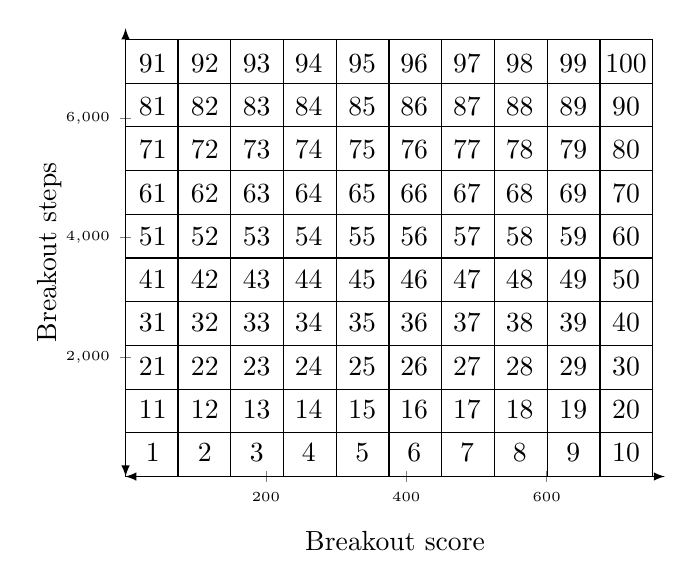
\begin{tikzpicture}
    
    \draw[step=1.0,black,thin,xshift=0cm,yshift=0cm,x=.67cm,y=.555cm] (0,0) grid (10,10);
    
    \node at (.35,.30) {1};
    \node at (1.01,.30) {2};
    \node at (1.67,.30) {3};
    \node at (2.33,.30) {4};
    \node at (3.01,.30) {5};
    \node at (3.67,.30) {6};
    \node at (4.34,.30) {7};
    \node at (5.01,.30) {8};
    \node at (5.69,.30) {9};
    \node at (6.36,.30) {10};
    
    \node at (.35,.85) {11};
    \node at (1.01,.85) {12};
    \node at (1.67,.85) {13};
    \node at (2.33,.85) {14};
    \node at (3.01,.85) {15};
    \node at (3.67,.85) {16};
    \node at (4.34,.85) {17};
    \node at (5.01,.85) {18};
    \node at (5.69,.85) {19};
    \node at (6.36,.85) {20};
    
    \node at (.35,1.4) {21};
    \node at (1.01,1.4) {22};
    \node at (1.67,1.4) {23};
    \node at (2.33,1.4) {24};
    \node at (3.01,1.4) {25};
    \node at (3.67,1.4) {26};
    \node at (4.34,1.4) {27};
    \node at (5.01,1.4) {28};
    \node at (5.69,1.4) {29};
    \node at (6.36,1.4) {30};
    
    \node at (.35,1.95) {31};
    \node at (1.01,1.95) {32};
    \node at (1.67,1.95) {33};
    \node at (2.33,1.95) {34};
    \node at (3.01,1.95) {35};
    \node at (3.67,1.95) {36};
    \node at (4.34,1.95) {37};
    \node at (5.01,1.95) {38};
    \node at (5.69,1.95) {39};
    \node at (6.36,1.95) {40};
    
    \node at (.35,2.5) {41};
    \node at (1.01,2.5) {42};
    \node at (1.67,2.5) {43};
    \node at (2.33,2.5) {44};
    \node at (3.01,2.5) {45};
    \node at (3.67,2.5) {46};
    \node at (4.34,2.5) {47};
    \node at (5.01,2.5) {48};
    \node at (5.69,2.5) {49};
    \node at (6.36,2.5) {50};
    
    \node at (.35,3.05) {51};
    \node at (1.01,3.05) {52};
    \node at (1.67,3.05) {53};
    \node at (2.33,3.05) {54};
    \node at (3.01,3.05) {55};
    \node at (3.67,3.05) {56};
    \node at (4.34,3.05) {57};
    \node at (5.01,3.05) {58};
    \node at (5.69,3.05) {59};
    \node at (6.36,3.05) {60};
    
    \node at (.35,3.6) {61};
    \node at (1.01,3.6) {62};
    \node at (1.67,3.6) {63};
    \node at (2.33,3.6) {64};
    \node at (3.01,3.6) {65};
    \node at (3.67,3.6) {66};
    \node at (4.34,3.6) {67};
    \node at (5.01,3.6) {68};
    \node at (5.69,3.6) {69};
    \node at (6.36,3.6) {70};
    
    \node at (.35,4.15) {71};
    \node at (1.01,4.15) {72};
    \node at (1.67,4.15) {73};
    \node at (2.33,4.15) {74};
    \node at (3.01,4.15) {75};
    \node at (3.67,4.15) {76};
    \node at (4.34,4.15) {77};
    \node at (5.01,4.15) {78};
    \node at (5.69,4.15) {79};
    \node at (6.36,4.15) {80};
    
    \node at (.35,4.7) {81};
    \node at (1.01,4.7) {82};
    \node at (1.67,4.7) {83};
    \node at (2.33,4.7) {84};
    \node at (3.01,4.7) {85};
    \node at (3.67,4.7) {86};
    \node at (4.34,4.7) {87};
    \node at (5.01,4.7) {88};
    \node at (5.69,4.7) {89};
    \node at (6.36,4.7) {90};
    
    \node at (.35,5.25) {91};
    \node at (1.01,5.25) {92};
    \node at (1.67,5.25) {93};
    \node at (2.33,5.25) {94};
    \node at (3.01,5.25) {95};
    \node at (3.67,5.25) {96};
    \node at (4.34,5.25) {97};
    \node at (5.01,5.25) {98};
    \node at (5.69,5.25) {99};
    \node at (6.36,5.25) {100};
    
    
    \begin{axis}[
        xmin=0,xmax=768,
        ymin=0,ymax=7500,
        axis lines=middle,
        enlargelimits={abs=0.5},
        axis line style={latex-latex},
        ticklabel style={font=\tiny,fill=white},
        x label style={at={(axis description cs:0.5,-0.1)},anchor=north},
        y label style={at={(axis description cs:-0.1,.5)},rotate=90,anchor=south},
        xlabel={Breakout score},
        ylabel={Breakout steps}
    ]
    
    \coordinate (O) at (0,0);
    
    \end{axis}
    \end{tikzpicture}
    
    \caption{ID de nicho en Breakout}
    \label{fig:brekaoutNichingID}
\end{figure}

\newpage